% This is the aspauthor.tex LaTeX file
% Copyright 2010, Astronomical Society of the Pacific Conference Series

\documentclass[11pt,twoside]{article}
\usepackage{asp2010}

\resetcounters
%\bibliographystyle{asp2010}
\markboth{K. Anderson, et al}{LOFAR and HDF5}
\begin{document}
\title{LOFAR and HDF5: Toward a New Radio Data Standard}
\author{Kenneth Anderson$^1$, A. Alexov$^1$, L. Baehren$^1$, J-M. Griessmeier$^2$,
M. Wise$^3$, G.A. Renting$^3$}
\affil{$^1$Astronomical Institute “Anton Pannekoek”, University of Amsterdam, 
Postbus 94249, 1090 GE Amsterdam, The Netherlands Institution}
\affil{$^2$Laboratoire de Physique et Chimie de l'Environnement et de l’Espace (LPC2E),
3A Avenue de la Recherche, 45071 Orléans Cedex 2, France}
\affil{$^3$Netherlands Institute for Radio Astronomy (ASTRON), Oude Hoogeveensedijk 4	 
7991 PD Dwingeloo, The Netherlands}
\begin{abstract}
For decades now, scientific data volumes have experienced relentless, exponential growth.
As a result, legacy astronomical data formats are straining under a burden not conceived
when these formats were first introduced. With future astronomical projects ensuring this
trend, ASTRON and the LOFAR project is exploring the use of the Hierarchical Data Format,
version 5 (HDF5), for LOFAR radio data encapsulation. Most of LOFAR's standard data products
will be stored natively using the HDF5 format. In addition, HDF5 analogues for traditional
radio data structures such as visibility data and spectral image cubes are also being developed.
The HDF5 libraries allow for the construction of potentially distributed, entirely unbounded files.
The nature of the HDF5 format further provides the ability to custom design a data encapsulation format.
The LOFAR project has designed several data formats that will accommodate all LOFAR data products, examples
of which are presented in this paper. With proper development and support,
it is hoped that these data formats will be adopted by other astronomical projects as they, too,
attempt to grapple with a future filled with mountains of data.
\end{abstract}
\section{Introduction}
The promising advent of the LOFAR telescope's operational epoch holds forth both great scientifiic
potential and challenges to current and legacy information technologies: volume and complexity of
the data will continue to push the envelope of commonly used data protocols.

Recognizing that this envelope is already strained, the LOFAR project has embarked on an ambitious
project to design and define a set of radio data standard formats that are capable of encapsulating
the full spectrum of, not just LOFAR data products, but astronomical radio data in general.

It is with this ambition in mind that the LOFAR data formats group have been developing these format
specifications and associated software infrastructure, an effort now ongoing for over two years.
It was determined that  HDF5 would be a robust, viable data framework that can handle the size, scope,
diversity, distributed nature and parallel I/O processing requirements of LOFAR data.
This work also has potential use beyond the radio community. New large scale optical telescopes
such as the LSST are also investigating the viability of using HDF5. Furthermore, the 20 year history
of HDF and its continuing use by NASA's earth orbiting/observing missions ensure broad, ongoing use
and support.

In addition to the format descriptions themselves, the LOFAR project is currently developing a set of
software tools for creating and working with these formats. The Data Access Library (DAL) in C++,
along with an associated Python interface (pyDAL), are designed to allow for the easy construction
and manipulation of these data formats. There are also a number of tools already available to read
and visualize HDF5 files, such as HDFView, ViSiT, PyTables, h5py and IDL.
\section{The LOFAR Radio Telescope}
Features of the LOFAR Radio Telescope, features that point to massive data volumes.\footnote{Image courtesy A. Alexov, et al, ADASS XX, BoF5,
\textit{Towards HDF5: Encapsulation of Large and/or Complex Astronomical Data}}
\begin{figure}[htbp]
  \centering
  \includegraphics[scale=0.52]{lofar_pointings.eps}
  \caption{The LOFAR ``Superterp,'' multiple concurrencies across beams, pointings, modes}
  \label{fig:lofarpoint}
\end{figure}
\begin{itemize}{\small
\item Currently, the “largest radio telescope in the world.”
\item 25,000 networked, passive phased array antennae, 36 fields in The Netherlands
\item International stations; Germany(5), Sweden(2), France(2), UK(1)
\item International Baselines to 1500 km; unlimited potential expansion.
\item Low Band Antenna (LBA) bandpass:10-90 MHz
\item High Band Antenna (HBA) bandpas:110-250 MHz.
\item Data Correlation: IBM Blue Gene/P supercomputer, Groningen, NL.
}
\end{itemize}
\section{LOFAR Data: Variety, Complexity, Volume}
Datasets produced by LOFAR observations will vary tremendously in size.  Images, Beam-formed data,
Transient Buffer board (TBB)  time-series data are expected to produce large files, with the beam-formed
and TBB potentially forming files of several tens of terabytes.
\begin{table}[hbt]
  \centering
  \begin{tabular}{|ccccc|}
    \hline
    \sc Exposure & \sc Number of & \sc Number of & \sc File Size  & \sc File Size  \\
    \sc Time     & \sc Subbands  & \sc Stations  & \sc Known Mode & \sc Search Mode \\
    \hline \hline
     1 min & 248 & 20 & 11.2GB & 244GB \\
\hline
     10 min & 248 & 30 & 112GB & 3.3TB \\
\hline
     1 hr  & 248 & 10 & 672GB & 6.7TB \\
     1 hr  & 248 & 20 & 672GB & 13.4TB\\
     1 hr  & 248 & 30 & 672GB & 26.8TB \\
\hline
     2 hr  & 248 & 5 & 1.3TB & 6.7TB \\
\hline
     12 hr & 248 & 5 & 8.0TB & 40.3TB \\
     12 hr & 248 & 15 & 24.0TB & 120.1TB \\
    \hline
 \end{tabular}
  \caption{Sample, LOFAR Beam-formed dataset sizes}
  \label{tab:data size}
\end{table}
LOFAR’s observational modes are capable of producing highly complex, large volume datasets. Indeed,
the path of diminishing utility of legacy protocols is clearly delineated.
This looming predicament is especially germane to the SKA pathfinder LOFAR project, wherein certain
operational modes will be capable of generating datasets comprising hundreds of gigabytes to tens of terabytes.
Therefore, the LOFAR project has been driven to consider viable alternatives to ``standard'' astronomical data formats,
such as FITS.  Though FITS development has sought to add capability to the protocol as needed (ESO-FWG, 2008),
such ex post facto approaches should not be expected to remain viable in the future.

Recognizing that legacy file technologies will eventually fail under the growing
demands of newer and larger scientific datasets, while simultaneously noting that
if observational modes of SKA pathfinder projects like LOFAR suggest anything,
it is that legacy technologies would have to be abandoned, not just because of
the volumes of data involved, but also because of the complex nature of the data per se.

\section{LOFAR Data Format Specifications}
A viable solution was needed for potentially massive LOFAR data products.
HDF5 provides a framework allowing users to essentially design their own files to
appropriately accommodate a known variety of data. The LOFAR project has been engaged in
developing and designing a complete set of specifications for all LOFAR observational data.
This has necessarily required differing file designs for differing data, with a certain
structural parallelism maintained across all file designs.

These Interface Control Documents4 (ICD) provide detailed descriptions of a range of expected LOFAR Data Products, including
Radio Sky Images, Transient Time Series data, Beam-Formed data, Dynamic Spectra, UV Visibility, Rotation Measure Synthesis, 
Near-field Imaging.  By way of example, the structure of a LOFAR Radio Sky Image file is outlined in the schematic diagram below.
\begin{figure}[htbp]
  \centering
  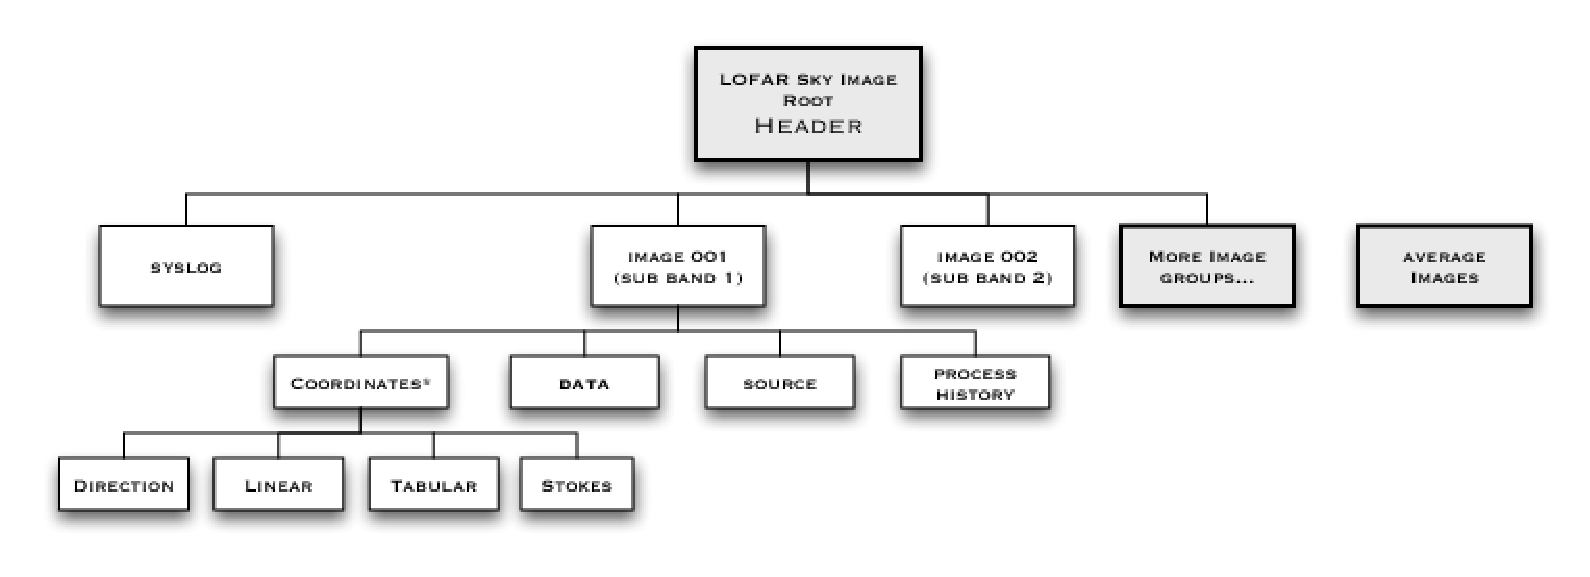
\includegraphics[scale=0.52]{SkyImDiag4.eps}
  \caption{LOFAR Radio Sky Image Data Structure}
  \label{fig:skyimDiag}
\end{figure}
\section{Summary and Future Considerations}
In order that adoption of HDF5 in astronomy prove useful in the real world,
the LOFAR project is committing resources to help develop the next generation of
astronomical tools for LOFAR data. The major effort at ATRON has been the development
of the Data Access Library (DAL), which ultimately will provide interfaces through FITS,
the Casa/AIPS++ Measurement Sets and HDF5. All LOFAR products will be accessible through DAL tools.

Ultimately we would like to see these formats grow into a true set of standards
for radio data that can meet the demands of the next generation of radio observatories.
Such standards are sorely lacking in the radio community at present and
something clearly needed as radio astronomy moves into the SKA era.

The effort by LOFAR to design an HDF5 radio data standard is primarily driven by two considerations.
One, there is no effective standard in radio astronomy data. Two, as indicated above, the expected
data volumes produced by LOFAR will, in many cases, swamp current file technology.  It is this reality
that has led LOFAR on this work, and it is hoped that these efforts toward building a radio data standard
will be recognized for the necessity it is, and one that is essential to the future development of radio astronomy.

\acknowledgements The author would like to thank colleagues at \textit{Sterrunkundig Instituut Anton Pannekoek},
the HDF Group, and the ADASS XX organization for what proved to be an excellent conference!

%\bibliography{aspauthor}

\end{document}
